\vspace{-10pt}
\section{Design and Implementation of \textsf{PCStream}}
\vspace{-5pt}

\begin{figure}[t]
	\centering
	%\vspace{-10pt}
	%\includegraphics[width=0.6\linewidth]{figure/architecture4}
	\includegraphics[width=0.7\linewidth]{figure/overview_1}
	\vspace{-9pt}
	\caption{An overall architecture of \textsf{\small PCStream}.}
	\label{fig:architecture}
	\vspace{-15pt}
\end{figure}

% stream tbl (X)
% 4.2 -> 5
% short-lived app (X)
% training?

In this section, we explain the detailed implementation of \textsf{\small
PCStream}.  Fig.~\ref{fig:architecture} shows an overall architecture of
\textsf{\small PCStream}. The \textit{PC Extractor} is implemented as
part of a kernel's system call handler as already described in
Section~\ref{sec:programcontext}, and is responsible for computing a PC signature
from applications.  
The PC signature is used for deciding the corresponding stream ID\footnote{
We call {\it i} the stream ID of $S_i$.} from the PC attribute table.
\textsf{\small PCStream} maintains various per-PC attributes in the PC attribute table
including PC signatures, expected data lifetimes, and stream IDs.
In order to keep the PC attribute table updated over changing workloads,
the computed PC signature with its LBA information is also sent to the 
{\it lifetime manager}, which 
estimates expected lifetimes of data belonging to given PCs.
Since commercial multi-streamed SSDs only expose a limited number of streams to a host, 
the \textit{PC2Stream mapper} groups PCs with similar lifetimes using a clustering
policy, assigning PCs in the same group to the same stream.  
Whenever the lifetime manager or the PC2Stream mapper are invoked,
the PC attribute table is updated with new outputs from these modules.
Finally, the
\textit{internal stream manager} implemented inside an SSD creates, removes,
and maintains internal streams associated with external streams.

%the lifetime of data written by write-related system calls can be
%monitored at the program context level.  
%A PC signature value is stored in an
%inode data structure of a file system (modified for \textsf{\small PCStream})
%and is delivered to \textit{the lifetime analyzer module} which estimates
%expected lifetimes of data belonging to a given PC in the block device level.
%In order to efficiently detect the end of data lifetime in append-only
%workloads, the lifetime analyzer also intercepts TRIM~\cite{TRIM} requests from
%a file system.

%shane part Based on the lifetime information, \textit{the PC-to-stream mapper
%module} clusters PCs with similar lifetimes and maps them together to the same
%stream ID.  This mapping is required because the number of streams in an SSD
%is generally less than the number of PCs in host applications.

\vspace{-10pt}
\subsection{PC Lifetime Management}
\vspace{-5pt}
The responsibility of the lifetime manager is for estimating the lifetime of
data associated with a PC. 
Except for outlier PCs, most data from the same PC tend to show similar 
data lifetimes with small variances.

\textbf{Lifetime estimation:}
Whenever a new write request {\it R} arrives, 
the lifetime manager stores the write request time,
the PC signature, $PC_i$, and the LBA list of {$R$} into the live LBA table.
The live LBA table, indexed by an LBA, is used in computing the lifetime of data stored
at a given LBA which belongs to $PC_i$.
Upon receiving TRIM commands (that delete previously written LBAs)
or overwrite requests (that update previously
written LBAs), the lifetime manager searches the live LBA table for a PC
signature $PC_{found}$ with the LBA list which includes the deleted/updated LBAs.
The new lifetime $l_{new}$ of $PC_{found}$ is estimated using the lifetime 
of the matched LBA from the live LBA table. The weighted average of the existing
lifetime $l_{old}$ for $PC_{found}$ and $l_{new}$ is used to update the $PC_{found}$
entry in the PC attribute table.
Note that the written time entry of the live LBA table is updated differently 
depending on TRIM commands or overwrite requests.
The written time entry becomes invalid for a TRIM command while it is updated by 
the current time for an overwrite request.

Maintaining the live LBA table, which is indexed by an LBA unit,
in DRAM could be a serious burden owing to its
huge size. In order to mitigate the DRAM memory requirement, 
the lifetime manager slightly sacrifices
the accuracy of computing LBA lifetime by increasing the 
granularity of LBA lifetime prediction to 1 MB, instead of 4 KB.  The
live LBA table is indexed by 1 MB LBA, and each table entry holds PC
signatures and written times over a 1-MB LBA range. 
Because of the coarse-grained indexing, each entry
could have multiple signatures and written times, and the same PC could span
across multiple entries.  If the same PC has different lifetimes, we take the
arithmetic mean as the PC lifetime. 
To limit the table size, if the table reaches a
threshold size, the least recently referenced entry is evicted from 
the LBA table.
In the current implementation, the threshold is set to 64 MB.
%For a 512 GB SSD with 1 MB-sized unit, assuming the table entry size is 48 B, 
%about 24 MB of host memory is required to hold the candidate table.

\textbf{PC attribute table:}
The PC attribute table keeps PC signatures and its expected lifetimes. To quickly
retrieve the expected lifetime of a requested PC signature, 
the PC attribute table is managed
through a hash data structure. Each hash entry requires only 12 bytes: 64-bit
for a PC signature and 32-bit for a predicted lifetime.  The table size is thus
quite small so that it can be entirely loaded in DRAM. 
From our evaluations, the DRAM size of the PC attribute table was sufficient 
with several tens of hundreds of KB.

In addition to the main function of the PC attribute table that maintains 
the data lifetime for a PC, the $memory-resident$ PC attribute table has 
another quite interesting benefit for the efficient
stream management.  Since a PC signature of an I/O activity is virtually 
guaranteed to be {\it unique} across {\it all} applications (the property 1),  
and a PC signature does not change over different executions of the same 
application (the property 2), the PC attribute table can capture a long-term 
history of programs' I/O behaviors.  
Because of the above two properties of a PC signature, \textsf{\small PCStream} can 
exploit the I/O behavior of even short-lived processes 
(e.g., cpp and cc1 for GCC)  that are launched and terminated frequently.  
When short-lived processes are frequently executed, the PC attribute table 
can hold their PC attributes from their previous executions, 
thus enabling quick but accurate stream allocation for short-lived
processes.

The property (2) is rather straightforward because each PC signature is 
determined by the sum of return addresses inside a process's
virtual address space.  Unless a program's binary is changed after
recompilation, those return addresses remain the same, regardless of program's
execution.  
The property (1) is also somewhat obvious from the observation
that the probability that distinct I/O activities that take
different function-call paths have the same PC signature is extremely low. This
is even true for multiple programs. Even though they are executed in the same
virtual address space, it is very unlikely that I/O activities of diverged
programs taking different function-call paths have the same PC.  
%We will show this in the experimental section. 
Consequently, this immutable property of
the PC signature for a given I/O activity makes it possible for us to characterize 
the given I/O activity in a long-term basis without a risk of PC collisions.

%The PC is determined by the sum of the return address, i.e., the path to reach
%the write system call.  In general, different I/O activities can not have the
%same return address because they are implemented in different functions.
%Since the probability that the sum of the different return addresses becomes
%the same is very low, the PC of an I/O activity in the same program is unique.
%For multiple programs, however, since each program uses a virtual address,
%several identical return addresses can occur.  However, the probability that
%two independent programs will have the same function call path over four or
%five is also very low, so we can usually say that a PC is unique.  Moreover,
%since the virtual address of the code is not changed after the compilation,
%the PC value will be the same when the program execution is terminated and
%restarted.  PCs of restarted program will be the same as the one of previous
%execution, and the life characteristics of the PC are also the same.  Because
%PCs are unique, if PC lifetime information is maintained, appropriate stream
%can be allocated even to the first request of a restarting program.

\vspace{-10pt}
\subsection{Mapping PCs to SSD streams}
\vspace{-5pt}

After estimating expected lifetimes of PC signatures, the PC2Stream mapper 
attempts to group PCs with similar lifetimes into an SSD stream.  This grouping
process is necessary because while commercial SSDs only support a limited number
of streams, the number of unique PCs can be quite large (e.g., 20).  
For grouping PCs with similar lifetimes, the PC2Stream mapper module uses the k-means
algorithm~\cite{kmeans} which is widely used for similar purposes.  
In \textsf{\small PCStream}, we use the difference in the data lifetime between two PCs 
as a clustering distance and  generates {\it m} clusters of PCs for $m$ streams.
This algorithm is particularly well suited for our purpose because 
it is lightweighted in terms of the CPU cycle and memory requirement.
To quickly assign a proper stream to incoming data, we add an extra field to the
PC attribute table which keeps a stream ID for each PC signature.  More
specifically, when a new write request comes, a designated SSD stream ID is
obtained by referring to the PC attribute table using request's PC value as an
index.  If there is no such a PC in the table, or a PC does not have a
designated stream ID, the request gets default stream ID, which is set to 0.

For adapting to changing workloads, re-clustering operations should be
performed regularly. This re-clustering process can be done in a
straightforward manner. The PC2Stream mapper scans up-to-date lifetimes for
all PCs in the PC attribute table. Note that PC's lifetimes are updated whenever
the lifetime manager gets new lifetimes while handling overwrites or TRIM requests,
as explained in Section 5.1.  With the scanned information, the PC2Stream mapper
recomputes stream IDs and updates stream fields of the PC attribute table.
In order to minimize unnecessary overhead of frequent re-clustering operations, 
re-clustering is triggered when 10\% of the PC lifetime entries in the PC attribute
table is changed.


\vspace{-10pt}
\subsection{Internal Stream Management}
\vspace{-5pt}
As explained in Section 4.1, there are a few outlier PCs with large lifetime
variances. In order to treat these PCs in an efficient fashion,
we devise a
two-phase method that decides SSD streams in two levels: the main stream in the
host level and its internal stream in the SSD level.  Conceptually, long-lived
data in the main stream are moved to its internal stream so that
(future) short-lived data of the main stream.  Although moving data to the
internal stream may increase WAF, the overhead can be hidden if we restrict
data copies to the internal stream during GC only.  Since long-lived data
(i.e., valid pages) in a victim block are moved to a free block during GC,
blocks belong to an internal stream tend to contain long-lived data.  For
instance, \textsf{\small PCStream} assigns the compaction-activity {\it
$PC_1$} to a main stream {\it $S_1$} in the first phase.  To separate the
long-lived data of {\it $PC_1$} (e.g., L4 data) from future short-lived data of
the same {\it $PC_1$} (e.g., L1 data), valid pages of the {\it $S_1$} are
assigned to its internal stream for the second phase during GC.

We have implemented the internal stream manager with the two-phase method in
Samsung's PM963 SSD~\cite{PM963}. To make it support the two-phase method, we
have modified its internal FTL so that it manages internal streams while
performing GC internally. 
Since the internal stream manager assigns blocks for an internal stream 
and reclaims them inside the SSD, no host interface changed is required.

%{\color{blue} 추가로, SSD가 지원하는 stream의 개수가 변경되는 상황에서도
%reclustering을 통해
%대응이 가능하다.
%reclustering의 주기는 workload의 변화 패턴에 따라 결정될 수 있다.
%새로운 PC가 계속적으로 생성되거나 한 PC의 수명 패턴이 자주 변화할 경우 reclustering의 주기를 
%좀 더 짧게 설정하여 workload 변화를 반영한다.
%}
%Since the
%number of PCs created by applications is not limited, the clustering algorithm
%must be efficient enough to quickly handle many PCs. 

\vspace{-10pt}
\subsection{PC Extraction for Indirect Writes}
\vspace{-5pt}
One limitation of using PCs to extract I/O characteristics is that it only
works with C/C++ programs that \textit{directly} call write-related system
calls.  Many programs, however, often invoke write system calls
\textit{indirectly} through intermediate layers, which makes it difficult to
track program contexts.

The most representative example may be Java programs, such as Cassandra and
Hadoop, that run inside a Java Virtual Machine (JVM). Java programs invoke
write system calls via the Java Native Interface (JNI)~\cite{JNI} that enables
Java programs to call native I/O library written in C and C++.
For Java program, therefore, the PC extractor shown in Fig.~\ref{fig:architecture} fails
to capture Java-level I/O activities because it is unable to inspect the JVM  
stack from the native write system call which is indirectly called through the JNI.
Another example is a program that maintains a write buffer that is
dedicated to dealing with all the writes from an application. For example, in
MySQL~\cite{MySQL} and PostgreSQL~\cite{PostgreSQL}, every write is first
sent to a write buffer. Separate flush threads later materialize buffered data
to persistent storage.  In that case, the PC extractor only captures PCs of
flush threads, not PCs of I/O activities that originally generate I/O requests,
because the I/O activities were executed in different threads using different
execution stacks.

\begin{figure}[t]
\centering
	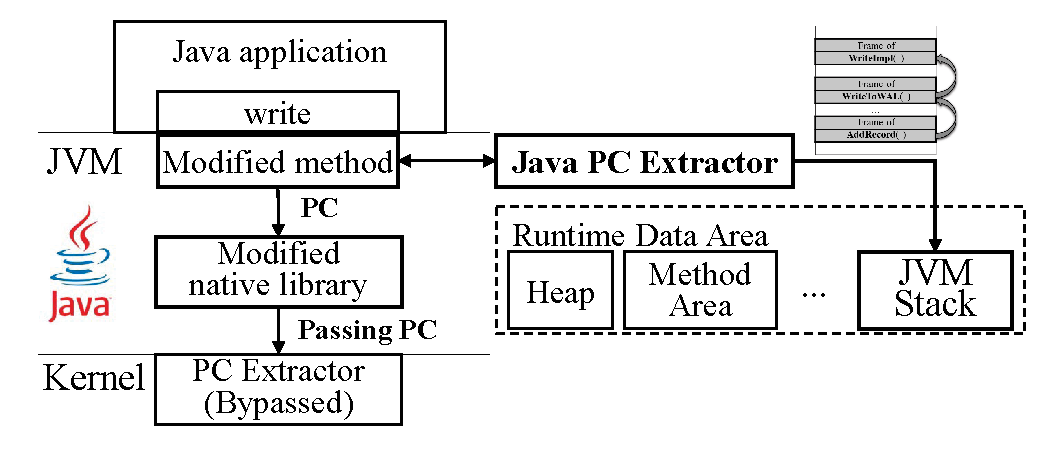
\includegraphics[width=0.7\linewidth]{figure/jvmpc}
	\vspace{-10pt}
	\caption{Extracting PCs for JVM.}
\label{fig:java}
	\vspace{-15pt}
\end{figure}


The problem of indirect writes can be addressed by collecting PC signatures 
{\it at the front-end interface} of an intermediate layer that accepts write requests
from other parts of the program. In case of Java programs, a native I/O library can
be modified to capture write requests and computes their PC signatures. Once a native
library is modified, \textsf{\small PCStream} can automatically gather PC signatures without modifying
application programs. Fig.~\ref{fig:java} illustrates how \textsf{PCStream}
collects PC signatures from Java programs.  We have modified the OpenJDK~\cite{OpenJDK} 
source to extract PC signatures for most of write methods in
write related classes, such as \texttt{OutputStream}.  The stack area in the
\texttt{Runtime Data Areas} of JVM was used to calculate PC signatures.  The
calculated PC is then passed to the write system call of the kernel via the
modified native I/O libraries.

Unlike Java, there is no a straightforward way to collect PCs from applications
with write buffers. This is because the implementation of write buffering is
different depending on applications. Thus, additional efforts to manually
modify code are unavoidable. However, the scope of this manual modification is
limited only to the write buffering code, and application logics themselves don't
need to be edited or annotated.


